% Activate the following line by filling in the right side. If for example the name of the root file is Main.tex, write
% "...root = Main.tex" if the chapter file is in the same directory, and "...root = ../Main.tex" if the chapter is in a subdirectory.
 
%!TEX root =  ../Thesis.tex

\chapter[Trigger and Cuts]{Trigger and Cuts}
\label{chap:trig_cuts}
The very first steps of any analysis consist of gathering the data, and then reducing the background
as much as possible.  For an experiment like ATLAS, with a dataset that approaches 3 PB of raw
data collected per year, picking a subset of that data for performing the search is both nontrivial
and crucial to the overall success of an analysis.  

The data selection starts with the trigger, which determines which events will even be recorded in the
first place.  The trigger must balance the competing forces of signal processes that can be very rare
(which would suggest a permissive trigger, so as to not lose already-rare signal events) and the
huge background rates at the LHC (which would suggest a strict trigger).  Since the trigger must make
decisions about event acceptance in near real-time, it can generally only require basic physics objects
like jets and $b$-tags, and more sophisticated background rejection gets implemented as offline event 
selection criteria, also called cuts.  

 
\section{Trigger}
\label{sec:my_trigger}
The purpose and structure of the ATLAS trigger are explained in Section~\ref{sec:atlas_trig}.
Most importantly for this section, recall that the ATLAS trigger has three levels, called L1,
L2, and EF.  The trigger chain for this analysis is as follows: 

\begin{itemize}
    \item L1: At least one J75 RoI\footnote{RoI stands for region of interest, an ATLAS acronym
    for a physical area in the calorimeter which has a large number of adjacent firing calorimeter
    cells, which collectively serve as a jumping-off point for a jet clustering algorithm}, implying an L1 jet of at least 75 GeV
    \item L2: least two 30 GeV jets, of which one must be at least 140 GeV. Additionally, at least two
jets must satisfy a medium $b$-tag (L2 xComb\footnote{xComb is the name of the $b$-tagging algorithm
that is used in the trigger} $>$ 1.276)
    \item EF: At least two 35 GeV jets, of which one must be at least 145 GeV. Additionally, at least two
jets must satisfy a medium $b$-tag (EF xComb\footnote{xComb is used in both L2 and EF of the trigger;
the values of the inputs to the algorithm can change between L2 and EF as more computationally intensive
reconstruction techniques are used in EF compared to L2} $>$ 1.099). There is no explicit requirement that the
$b$-tagged jets from L2 correspond with the $b$-tagged jets from EF. However, as detailed later, this
requirement is added later as an offline cut.
\end{itemize}


In the trigger, the L2 and EF jets are b-tagged using xComb, a likelihood ratio of IP3D\footnote{IP3D, like
the other algorithms described here, uses statistical learning algorithms trained on a large sample
of Monte Carlo simulation events to predict whether a given jet is a $b$-jet or not.  The various $b$-taggers
vary in the algorithm and input features, which are very briefly summarized in this list. } 
(significance of $z_0$ and $d_0$ impact parameters), SV1 (mass of the secondary vertex), NVTX (the number of
vertices with two tracks), and EVTX (the energy fraction of the secondary vertex), as well as the number
of vertices with 2 tracks. 
The online $b$-tagging cuts used in the trigger for this analysis operate at the so-called ``loose''
working point, where the $b$-jet efficiency
is 70\%.

Table~\ref{tab:online_offline_btag} below shows the correlations between the two levels of online
$b$-tagging, as well as the offline (MV1) $b$-tagging for three offline working points (60\%, 70\%,
80\%).  

  \begin{table}[hbt]
\caption{  The acceptance of a cut on variable X given that the events have
  already passed (sig-like) or failed (bkgd-like) a cut on variable Y.\label{tab:online_offline_btag}}
    
    \begin{center}
    \begin{tabular}{l | l | c | c || c | c } \hline \hline
    \multicolumn{2}{c}{}  & \multicolumn{2}{c}{Signal MC} & \multicolumn{2}{c}{Unbiased Data} \\ \hline
      X         & Y         & sig-like & bkgd-like   &   sig-like & bkgd-like \\
      \hline
      EF        & L2        & 0.917    & 0.248 &   0.424       & 0.035 \\
      \hline
      L2        & MV1 (80)  & 0.675    & 0.031 &       0.510       & 0.077 \\
      EF        & MV1 (80)  & 0.824    & 0.090 & 0.515       & 0.050\\
      L2 and EF & MV1 (80)  & 0.676    & 0.036 & 0.414       & 0.031 \\
      MV1 (80)  & L2 and EF & 0.977    & 0.434 & 0.640       & 0.076 \\
      \hline
      L2        & MV1 (70)  & 0.716    & 0.060 & 0.652       & 0.086\\
      EF        & MV1 (70)  & 0.867    & 0.131 & 0.665       & 0.060 \\
      L2 and EF & MV1 (70)  & 0.721    & 0.060 & 0.563       & 0.038\\
      MV1 (70)  & L2 and EF & 0.954    & 0.340 & 0.538       & 0.034\\
      \hline
      L2        & MV1 (60)  & 0.757    & 0.101 & 0.762       & 0.095\\
      EF        & MV1 (60)  & 0.903    & 0.193 & 0.779       & 0.070 \\
      L2 and EF & MV1 (60)  & 0.765    & 0.103 & 0.692       & 0.045\\
      MV1 (60)  & L2 and EF & 0.902    & 0.250 & 0.429       & 0.015\\ \hline
    \end{tabular}
    \\
    \vspace{2mm}
    \end{center}
  \end{table}
  


%------------------------------------------------------
\begin{figure}
    \center
	\begin{subfigure}[L2 and EF $b$-tags]{0.45\textwidth}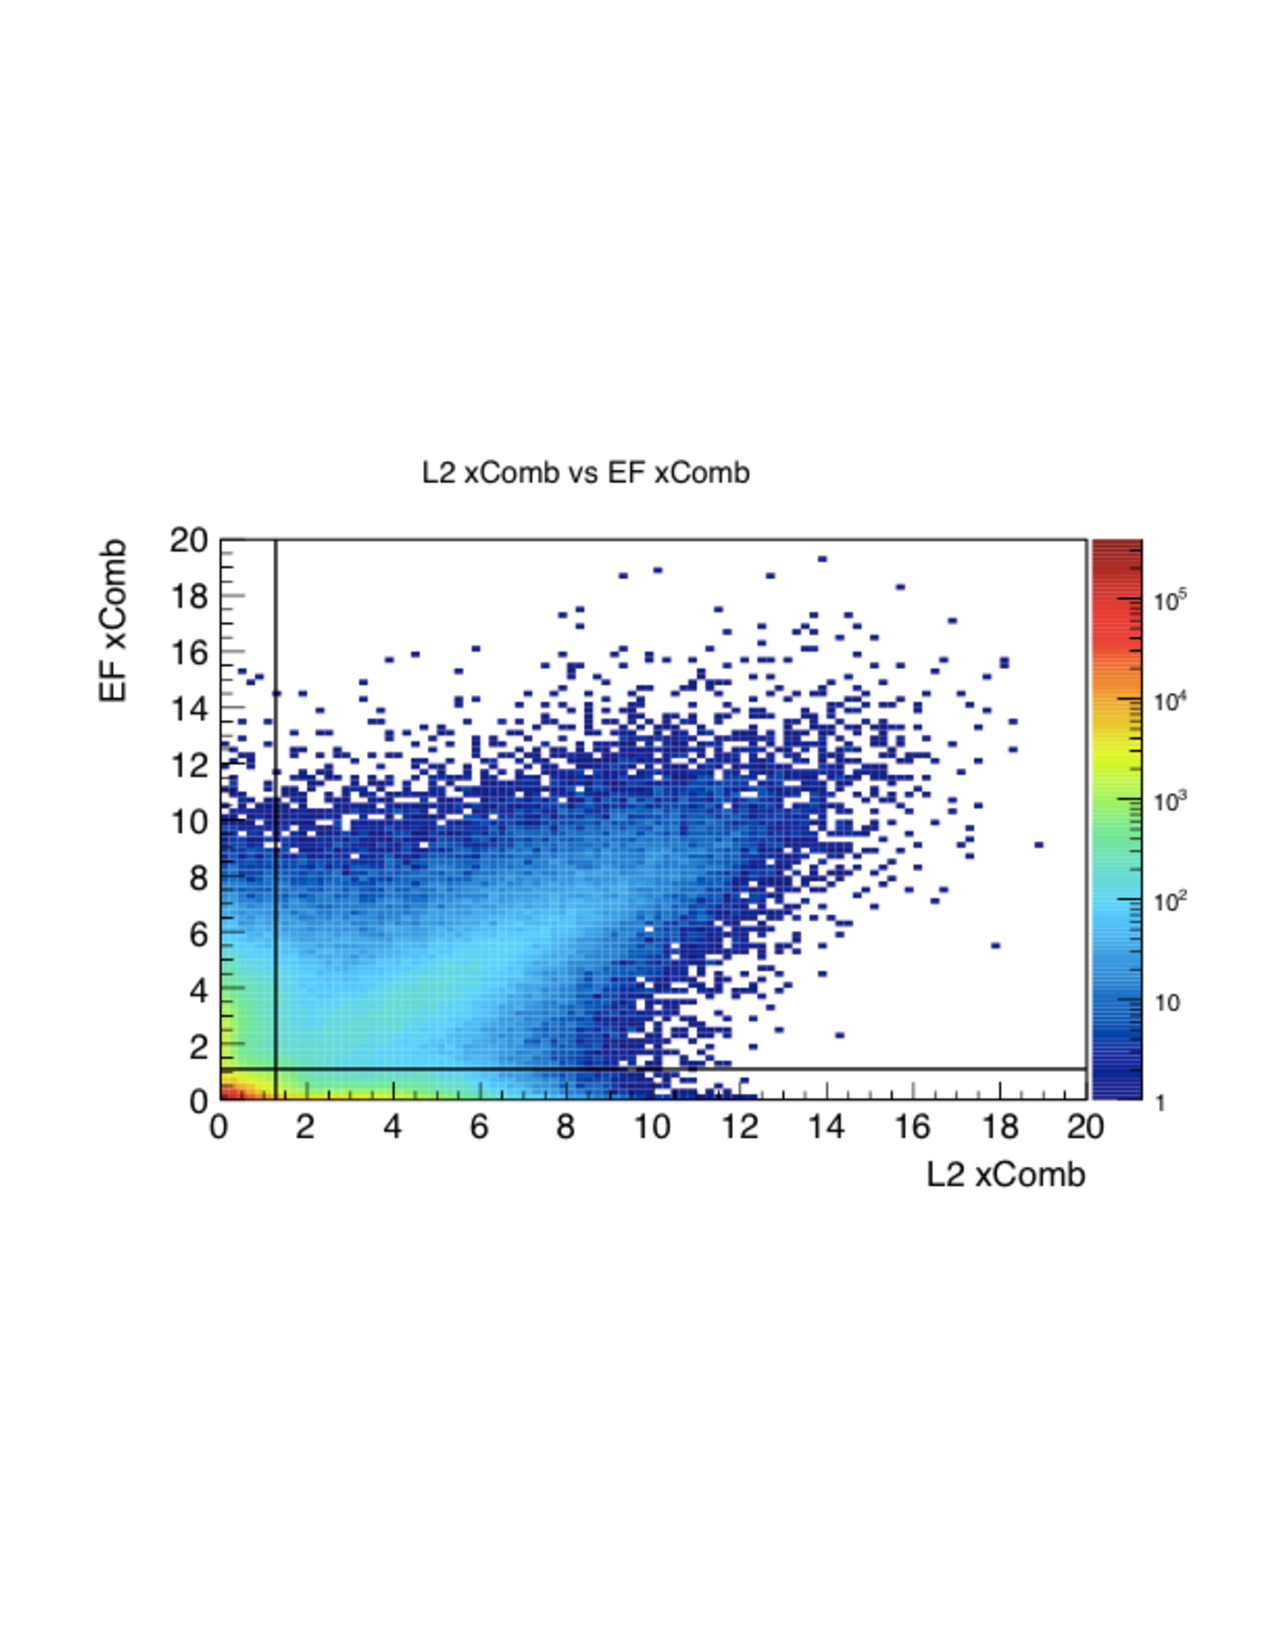
\includegraphics[width=\textwidth]{TriggerCuts/L2_EF.pdf}\end{subfigure}
	\begin{subfigure}[EF and MV1 $b$-tags]{0.45\textwidth}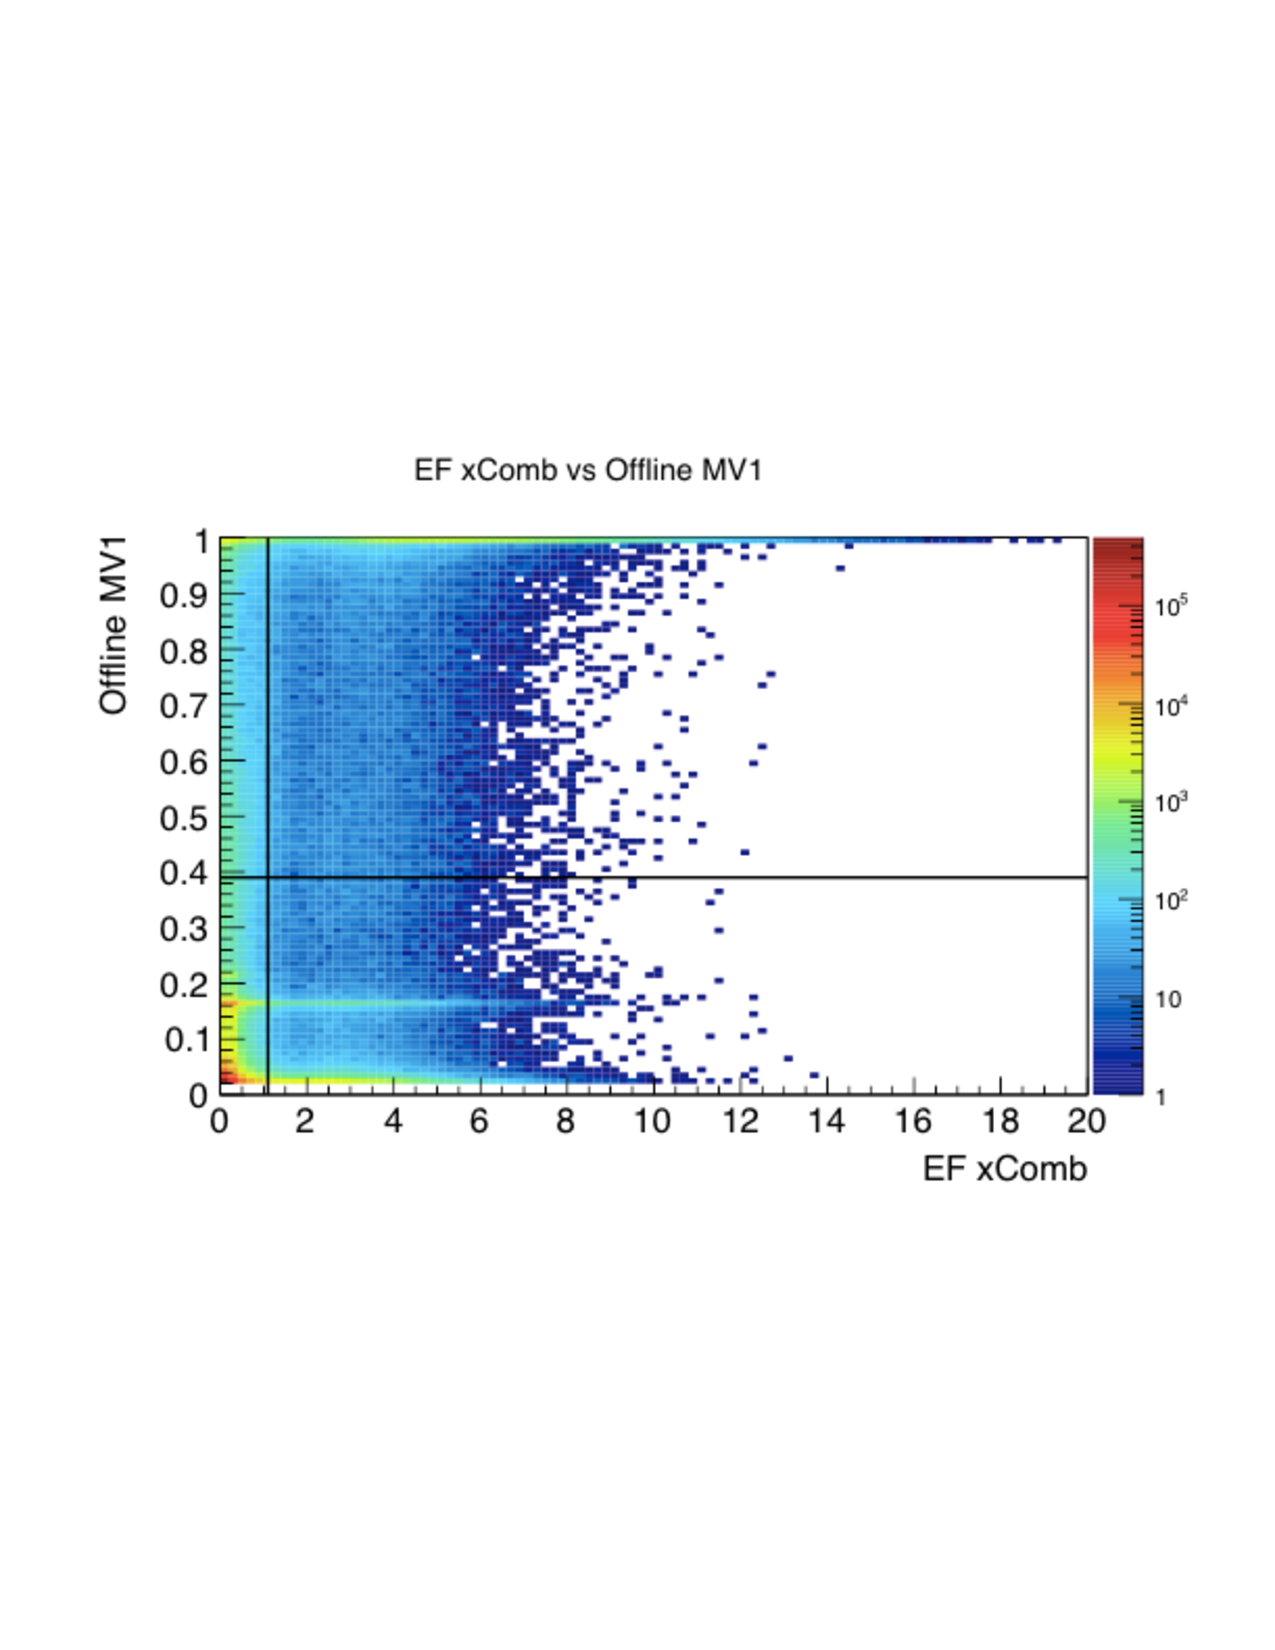
\includegraphics[width=\textwidth]{TriggerCuts/EF_MV1.pdf}\end{subfigure}
%  \begin{subfigure}[$m_{A}=550$ GeV]{0.4\textwidth}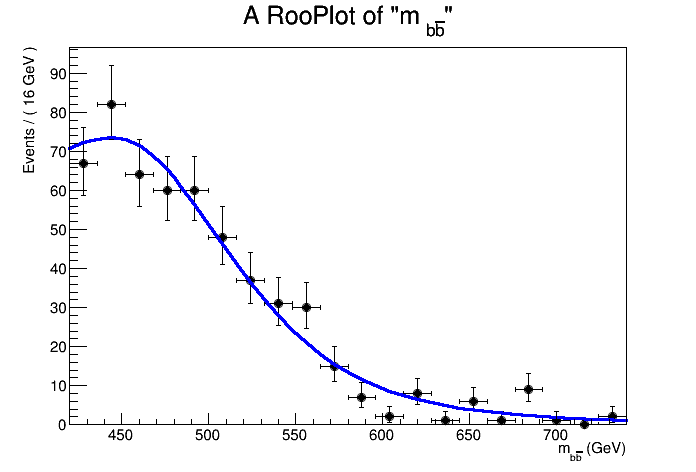
\includegraphics[width=\textwidth]{FitResults/images/fitMC_bAbb550_6.png}\end{subfigure}
    \caption{The $b$-tagging in Level 2 and 
    the Event Filter (in the trigger) and the MV1 $b$-tagging algorithm
    (offline) are exploited in the cut flow by requiring that at least
    2 jets in the event be ``triple tagged'', or $b$-tagged in both
    stages of the triggers as well as offline.  The figure on the
    left shows the L2 and EF $b$-tag distributions, on the right are the
    EF and MV1 distributions.  The cut points are noted with vertical
    and horizontal lines.  Most of the events (more than 80\%) fall
    in regions where the $b$-tagging cuts agree on whether a jet is 
    a $b$-jet or not, but a significant subsample of jets are tagged by 
    on $b$-tagging level/algorithm but not the other(s). \label{fig:L2_EF}}
\end{figure}

%------------------------------------------------------










\section{Offline Cuts}

Once an event has fulfilled the trigger requirements and been written to disk,
it must pass a series of offline cuts before being used in the final fit and search. 

\begin{itemize}
\item
\textbf{$p_T$ cuts of 155 and 55 GeV on leading and sub-leading jets, respectively.}
In order to get out of the \pt turn-on curves of the trigger, cuts of
155~GeV and 55~GeV are applied to the leading and second jets in the
event.
\item
\textbf{$p_T$ cut of 25 GeV on third jet.}
A third jet is not required by the trigger, but is required by
the offline cuts, and it must have a \pt greater than 25 GeV.  There is
no veto on additional jets.  Further details on the jet cuts can be found
in Section~\ref{sec:jet_reco}.
\item
\textbf{$\eta$ cuts on the leading 3 jets}
The leading three jets must be central, with $|\eta|<$2.5.  This is strongly
motivated by the $b$-tagging requirements downstream; the inner tracker only 
provides precision tracking out to $|\eta|<$2.5, which propagates through
to where $b$-tags can be computed and applied.
\item
\textbf{Two jets passing online (L2 and EF in trigger) and offline (MV1) $b$-tags}
As part of the trigger, two jets are required to be $b$-tagged at L2 and at EF.  It
is not explicitly required by the trigger that the same jets pass $b$-tagging at the two trigger levels,
or that those jets be tagged offline by the MV1 algorithm, so we make an
offline cut that imposes that requirement.  There is further discussion of the online
and offline $b$-tagging correlations in Section~\ref{sec:online_btagging},
where one of the important conclusions is that there is not perfect correspondence
between jets passing the three levels of $b$-tagging (L2, EF, MV1).  For
example, a jet with a large xComb value at L2 (and passing the $b$-tagging
requirement at L2) might have a small xComb value at EF (and fail the $b$-tagging
requirement at EF).  Likewise with L2 and MV1, or EF and MV1.  As a result, we
make an explicit requirement offline that the same two jets be $b$-tagged in L2, EF
and MV1.  Jets that are tagged in both L2 and EF of the trigger are referred to as
``trigger-tagged'' jets, and jets that pass L2, EF and MV1 are called ``triple-tagged''
jets.
The offline cut on the
trigger-matched $b$-jets is set to the 60\% efficiency
operating point. Due to the bias introduced by the trigger (see
Table~\ref{tab:online_offline_btag}), this provides additional rejection of
light jets for a relatively small decrease in signal efficiency.


\item\textbf{Leading 2 jets must pass tight MV1 $b$-tag}
We also require that the two jets in the event with the highest \pt be $b$-tagged
offline by the MV1 algorithm.  There is no explicit requirement that the leading
two jets be trigger-tagged or triple-tagged.
  In addition to preferentially keeping signal events at a higher rate than
background events, this cut considerably improves the combinatorics of reconstructing
the Higgs and we see markedly better signal mass peak resolution when this cut is in
place.  Further details can be found in Section~\ref{sec:combinatorics}.


\item
\textbf{Categorization based on $b$-tagging of a 3rd jet}
After two
$b$-jets have been triple-tagged, the event is categorized based on whether
a third $b$-tagged jet is present.  The most signal-enriched region is where
a third jet passes a tight (60\% efficiency) MV1 $b$-tag (\textit{bbb} category); the next most
signal-enriched region is when no jets in the event pass a 60\% $b$-tag
but there is at least one jet passing a loose (80\% efficiency) $b$-tag (\textit{bbloose} category);
the least sensitive region has no additional jets passing either 60\% or 
80\% $b$-tags (besides the triple-tagged jets, \textit{bbanti} category).  These tag categories are
mutually exclusive and all have different signal enrichments, kinematics, 
and provide varying levels of sensitivity when used in the fit (Section~\ref{sec:background_strategy}).
If there are more than three jets in an event, the event is categorized
by the most $b$-like (highest $b$-tag-weighted) jet in the event\footnote{for
example, an event with four jets total, three of which pass tight $b$-tags,
will be categorized as \textit{bbb}}).  If there are more than five
jets in an event, only the leading five are considered when assigning that event
to a $b$-tag category.


\item
\textbf{Categorization based on the number of jets in the event}
Similarly, the events are categorized into 3-jet, 4-jet, and 5 (or more) jet
categories, primarily because the varying signal resolution in the different
jet bins leads to different signal to background ratios, and separating
the categories allows for extra sensitivity to be extracted (Section~\ref{sec:n_jets_sig}).
Only jets with $p_T>$25 GeV and $|\eta|<$2.5 are considered when counting jets.
%The light-jet efficiency for this working point is approximately 0.1\%, and the
%charm efficiency is approximately 10\%.

\item 
\textbf{Rotation into Eigenbasis, and $p_T^{'}$ cuts}
After all the preceding precuts and categorizations are applied, the events
are rotated into a new basis based on the eigenvectors of the matrix composed of the
signal $m_{bb}$ and the $p_T$s of the leading 2 jets in the event.  Then cuts
based on the new (rotated) $p_T$s of the jets are applied, and the rotated $m_{bb}$
is used as the final discriminating variable.  Much more detail about this procedure,
its motivation and results, can be found in Section~\ref{sec:rotation}).



\end{itemize}



%------------------------------------------------------
\begin{figure}
    \center
	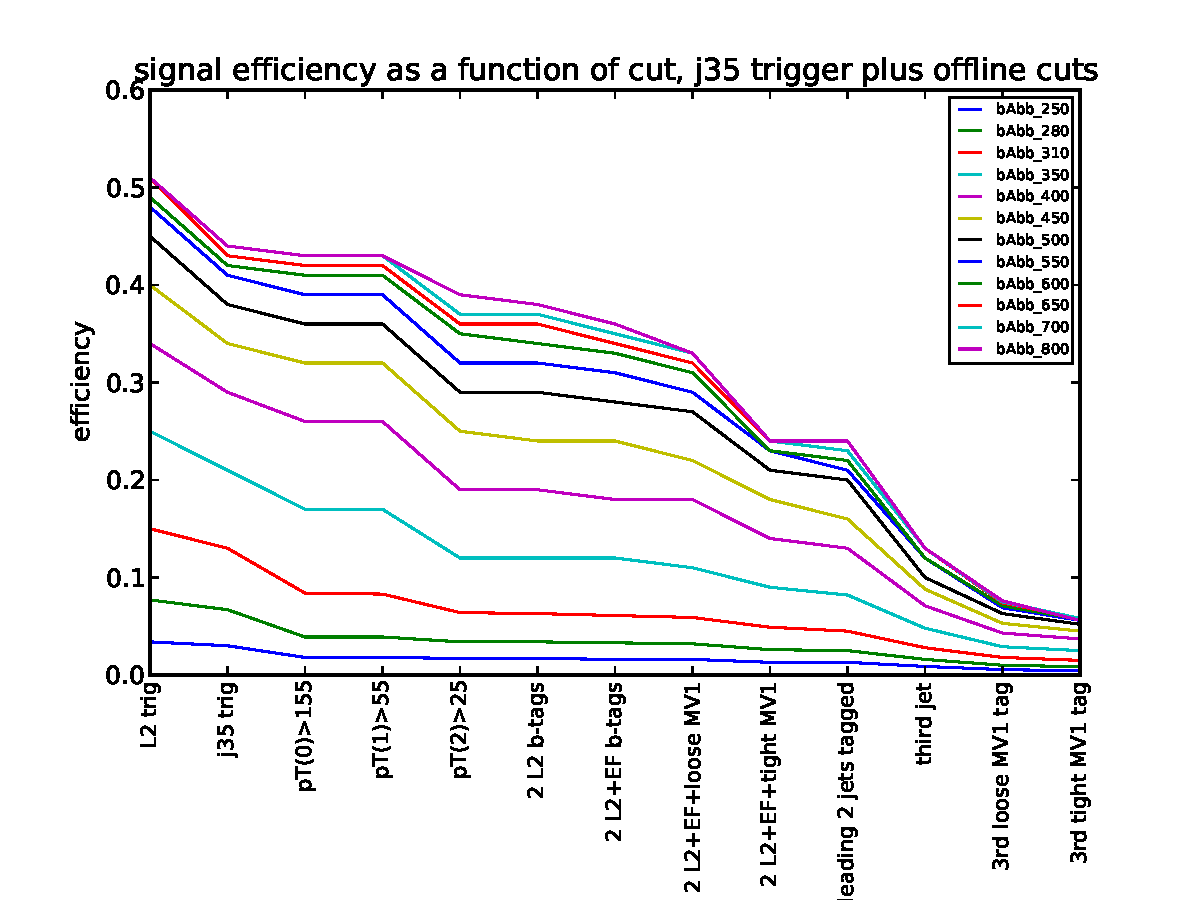
\includegraphics[width=0.98\textwidth]{TriggerCuts/cut_efficiencies_j35_signal.pdf}	
%	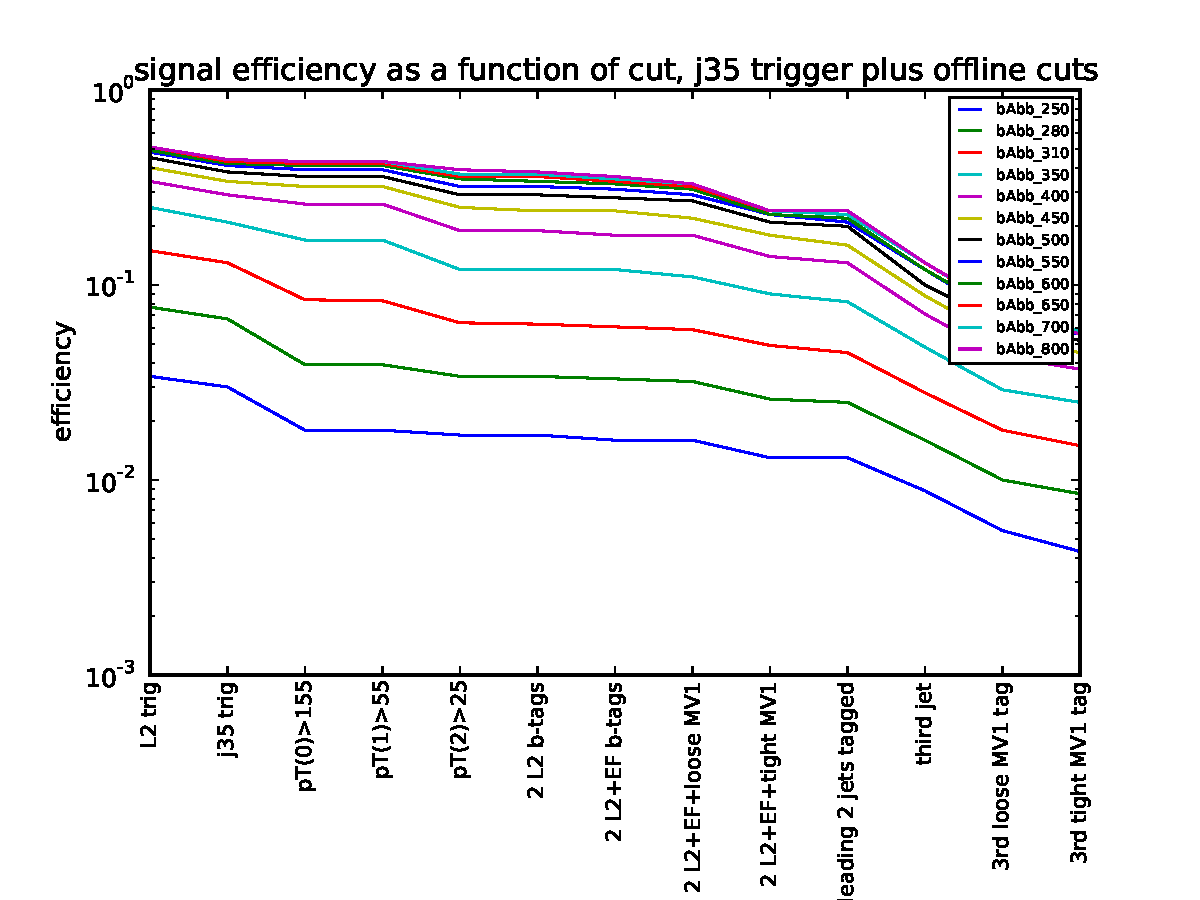
\includegraphics[width=0.98\textwidth]{TriggerCuts/cut_efficiencies_logy_j35_signal.pdf}	
    \caption{The cut efficiencies in signal, cut by cut.  Each line is a different
    signal mass point, and the overall trend is for higher efficiencies for the higher-mass
    particles than for the lower-mass particles. \label{fig:signal_eff_cutflow}}
\end{figure}

%------------------------------------------------------





%------------------------------------------------------
\begin{figure}
    \center
	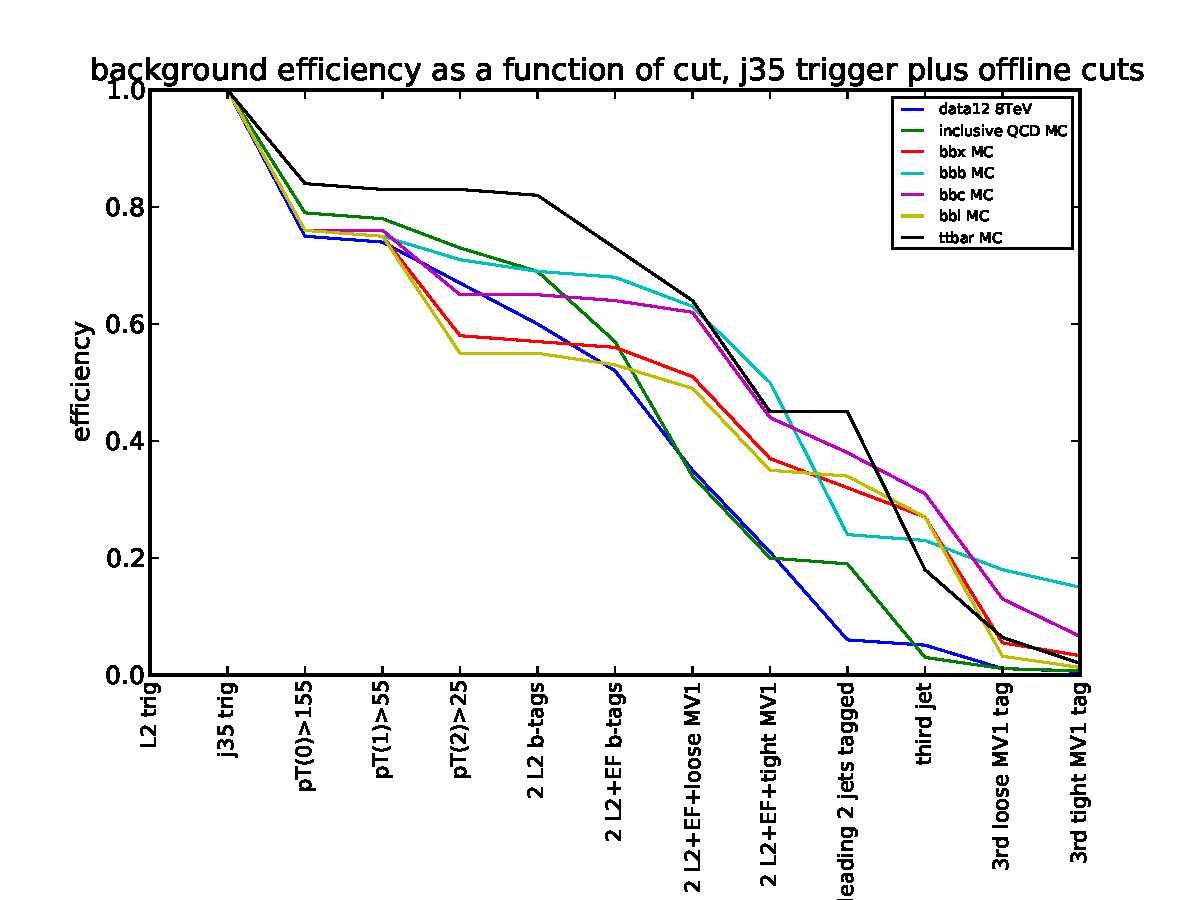
\includegraphics[width=0.98\textwidth]{TriggerCuts/cut_efficiencies_j35_background.pdf}	
%	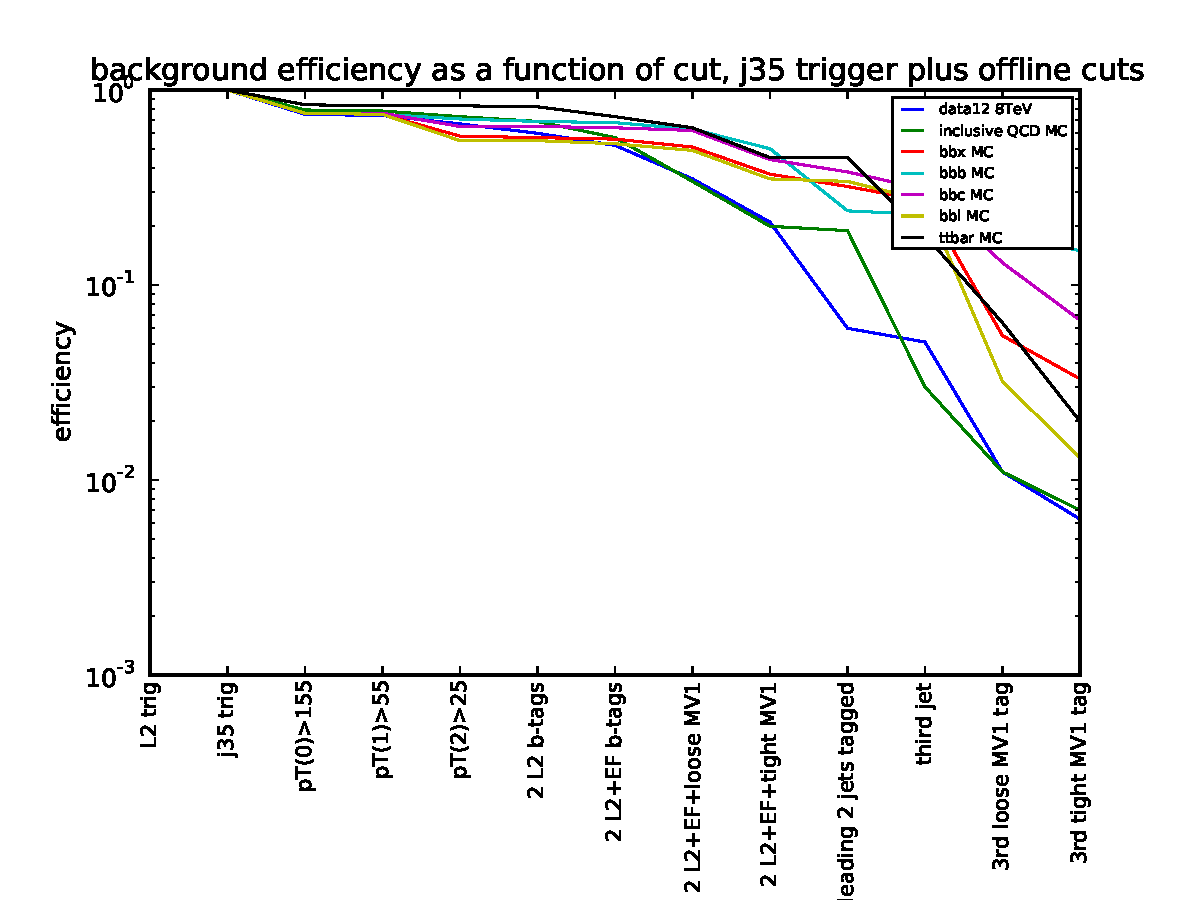
\includegraphics[width=0.45\textwidth]{TriggerCuts/cut_efficiencies_logy_j35_background.pdf}	
    \caption{The cut efficiencies in background, cut by cut. The background component that has 
    three real $b$-jets from QCD has the greatest survival rate through the cut flow, followed
    by events that have two $b$-jets and one $c$-jet.\label{fig:background_eff_cutflow}}
\end{figure}

%------------------------------------------------------

%------------------------------------------------------
\begin{figure}
    \center
	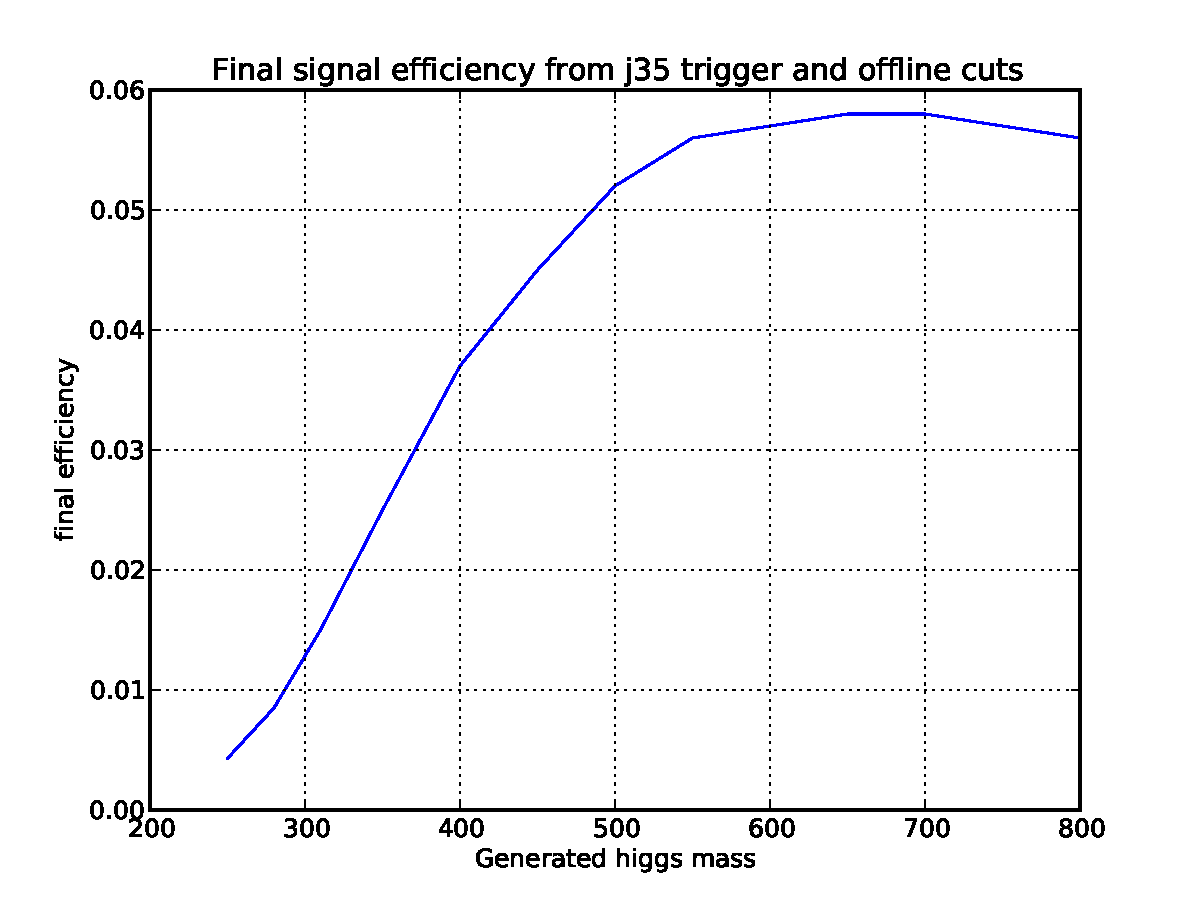
\includegraphics[width=0.98\textwidth]{TriggerCuts/final_efficiency_vs_mass_j35.pdf}	
    \caption{The final efficiency, after all cuts, of the signal as a function of
    the physical mass of the generated Higgs particle.  The signal efficiency grows as a
    function of $m_A$, although at the high mass values, the efficiency levels off at around 6\%.\label{fig:final_eff_vs_mass}}
\end{figure}

%------------------------------------------------------







